\section{Official Milestone}
\label{sec:OfficialMilestone}

The following is the ASC milestone our work implements.

\begin{quotation}

ASC calculations produce complex datasets that are increasingly difficult to explore and understand using traditional post-processing workflows.  To advance understanding of underlying physics, uncertainties, and results of ASC codes, SNL must gather as much relevant data as possible from large simulations.  This drives SNL to couple data analysis and visualization capability with a running simulation, so that high fidelity data can be extracted and written to disk.  This Milestone evaluates two approaches for providing such a coupling:

\begin{enumerate}
\begin{item}
In-situ processing provides ``tightly-coupled'' analysis capabilities through libraries linked directly with the simulation.  SNL has collaborated on developing an in-situ capability designed for this purpose.
\label{tightly-coupled-approach}
\end{item}
\begin{item}
In-transit processing provides ``loosely-coupled'' analysis capabilities by performing the analysis on separate processing resources.  SNL provides this capability through a ``data services'' capability designed for this purpose.
\label{loosely-coupled-approach}
\end{item}
\end{enumerate}

SNL will engineer, test and evaluate customer-driven operations on large-scale data created by a running simulation.  The data operations will be performed by instrumented versions of both the in-situ and in-transit solutions, with the resulting performance data published and made available to the ASC community.

A program review will be conducted, and its results documented.  A report will be submitted as a record of milestone completion.

\end{quotation}

Our ``customer-driven operations'' are encapsulated in the use case given
in Section~\ref{sec:UseCase}, which is designed by Jason Wilke, one of our
customers in Mechanical Engineering, to represent a typical shock physics
analysis.

The results of our instrumentation on the coupled simulation and \vda are
given in Section~\ref{sec:Results}.  These results come from experimental
runs on the Cielo supercomputer\lcite{Doerfler2011} ranging up to over 64
thousand cores.  Our measurements record the cost of coupling \vda to a
running simulation in terms of added execution time and memory overhead,
which satisfies the deliverables of the milestone.

The milestone describes ``two approaches'' for coupling a simulation with
\vda.  These approaches refer to the workflow employed in the full process
from simulation to data analysis.  These workflows are summarized in
Figure~\ref{fig:Workflows}.

\begin{figure}
  \centering
  \subfloat
      [Traditional offline post-processing \vda.]
      {
        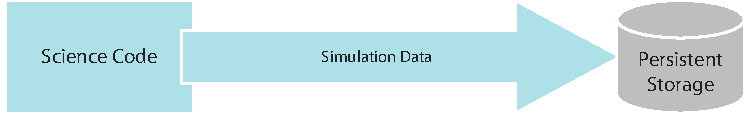
\includegraphics{figures/WorkflowsOffline}
        \label{fig:Workflows:Offline}
      } \\
  \subfloat
      [Embedded \insitu \vda (VDA).]
      {
        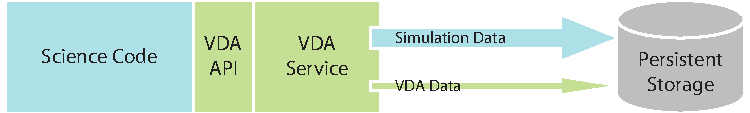
\includegraphics{figures/WorkflowsInSitu}
        \label{fig:Workflows:InSitu}
      } \\
  \subfloat
      [Service-oriented \intransit \vda (VDA).]
      {
        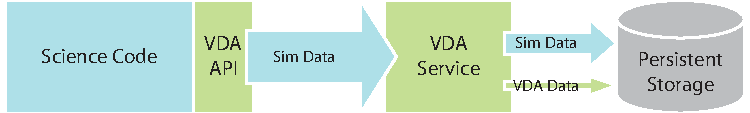
\includegraphics{figures/WorkflowsInTransit}
        \label{fig:Workflows:InTransit}
      }
  \caption[Visualization and data analysis workflows.]{Traditional and
    emerging workflow diagrams showing the flow of information from
    simulation to persistent storage.  In all cases data will later be
    retrieved from storage and further analyzed.}
  \label{fig:Workflows}
\end{figure}

The workflow in Figure~\ref{fig:Workflows:Offline} is a traditional
\keyterm{offline post-processing} in which the simulation stores all its
results to disk for later \vda.  This is what the milestone means by the
``traditional post-processing workflows'' with which ``complex
datasets... are increasingly difficult to explore and understand.''
Approach~\ref{tightly-coupled-approach} of the milestone refers to the
\keyterm{embedded \insitu} workflow in Figure~\ref{fig:Workflows:InSitu} in
which a \vda library is coupled with the running simulation code.
Approach~\ref{loosely-coupled-approach} of the milestone refers to the
\keyterm{\intransit} workflow in Figure~\ref{fig:Workflows:InTransit} in
which data is transfered from the simulation job to a separate \vda
service.

All three workflows are considered in our measurements.  The offline
post-processing workflow is implemented using the standard CTH I/O to write
full meshes to storage and then reading those meshes in a scripted parallel
ParaView job.  The embedded \insitu workflow is implemented with the
\keyterm{Catalyst} \insitu library discussed in Section~\ref{sec:Catalyst}.
The \intransit workflow is implemented with the \keyterm{Nessie} I/O
service described in Section~\ref{sec:Nessie}.
